\chapter{Genetic Algorithm: Milestone 4}
\section{Implementation}
The existing task allocation and routing formulation is retained. A chromosome has $2n$ random keys: $n$ allocation keys and $n$ sequence keys. Decoding assigns every task once and sorts each vehicle route by sequence key. Routes depart from and return to the depot.
The population contains 60 individuals, half generated by randomized insertion and half by random keys. Selection uses tournaments of size three. Uniform crossover is applied with probability 0.9. Each gene is independently reset with probability 0.05. Two elites survive unchanged. Incompatible allocation genes are resampled among compatible vehicles. Payload, battery and deadline violations remain explicitly evaluated.
Feasible individuals rank before infeasible individuals. Within the feasible set, the objective is $F=0.5T_{\mathrm{mission}}/T_{\max}+0.5E_{\mathrm{total}}/\sum_k B_k$. Infeasible individuals rank by normalized violation and then objective. This is a scalar optimization algorithm.
\section{Experimental design}
Each configuration uses five solver seeds on a fixed instance with generator seed zero. The evaluation budget is 3000, including initialization. SA uses 60 construction trials and 20 calibration samples, followed by at most 2920 proposals. Failed proposals can leave its evaluation count below the budget. Runtime includes initialization; SA caches unchanged routes, so evaluation count alone is not an equal-runtime comparison.
Six synthetic scale and constraint cases retain the previous milestone generator. Exact feasible optima are independently enumerated for six and seven tasks. These validate the implementation without claiming that synthetic cases reproduce published datasets. Parameter studies vary population, crossover and mutation one factor at a time under the same evaluation budget.
\section{Measured results}
Objective, mission time and energy summaries include feasible runs only. Feasibility rate includes every run. Raw runs, constraint violations, per-run routes, runtime and evaluation counts are supplied in the accompanying CSV and JSON files.
\begin{small}\begin{longtable}{llrrrr}
Case & Solver & Feasible & Mean $F$ & Time (s) & Gap (\%) \\ \hline
battery75 & GA & 0\% & -- & 6.2279 & -- \\
battery75 & SA & 0\% & -- & 6.9173 & -- \\
crossover\_0.6 & GA & 100\% & 0.2294 & 1.4322 & -- \\
crossover\_0.9 & GA & 100\% & 0.2308 & 1.4812 & -- \\
crossover\_1.0 & GA & 100\% & 0.2314 & 1.5370 & -- \\
exact6 & GA & 100\% & 0.2252 & 1.6738 & 0.0000 \\
exact6 & SA & 100\% & 0.2252 & 3.9443 & 0.0000 \\
exact7 & GA & 100\% & 0.2821 & 1.6266 & 0.0000 \\
exact7 & SA & 100\% & 0.2821 & 2.9316 & 0.0000 \\
gao100 & GA & 100\% & 0.5876 & 3.9857 & -- \\
gao100 & SA & 100\% & 0.4454 & 4.4838 & -- \\
gao50 & GA & 100\% & 0.5902 & 4.8569 & -- \\
gao50 & SA & 100\% & 0.5798 & 5.0514 & -- \\
mutation\_0.01 & GA & 100\% & 0.2246 & 1.3806 & -- \\
mutation\_0.05 & GA & 100\% & 0.2308 & 1.5944 & -- \\
mutation\_0.15 & GA & 100\% & 0.2314 & 3.0383 & -- \\
population\_120 & GA & 100\% & 0.2248 & 1.6747 & -- \\
population\_30 & GA & 100\% & 0.2278 & 1.2581 & -- \\
population\_60 & GA & 100\% & 0.2308 & 1.5361 & -- \\
reference30 & GA & 100\% & 0.2308 & 3.8375 & -- \\
reference30 & SA & 100\% & 0.2146 & 4.0388 & -- \\
restricted90 & GA & 100\% & 0.6014 & 4.4260 & -- \\
restricted90 & SA & 100\% & 0.5597 & 4.0891 & -- \\
small10 & GA & 100\% & 0.3184 & 3.9088 & -- \\
small10 & SA & 100\% & 0.3184 & 34.0126 & -- \\
\end{longtable}\end{small}
\begin{figure}[htbp]\centering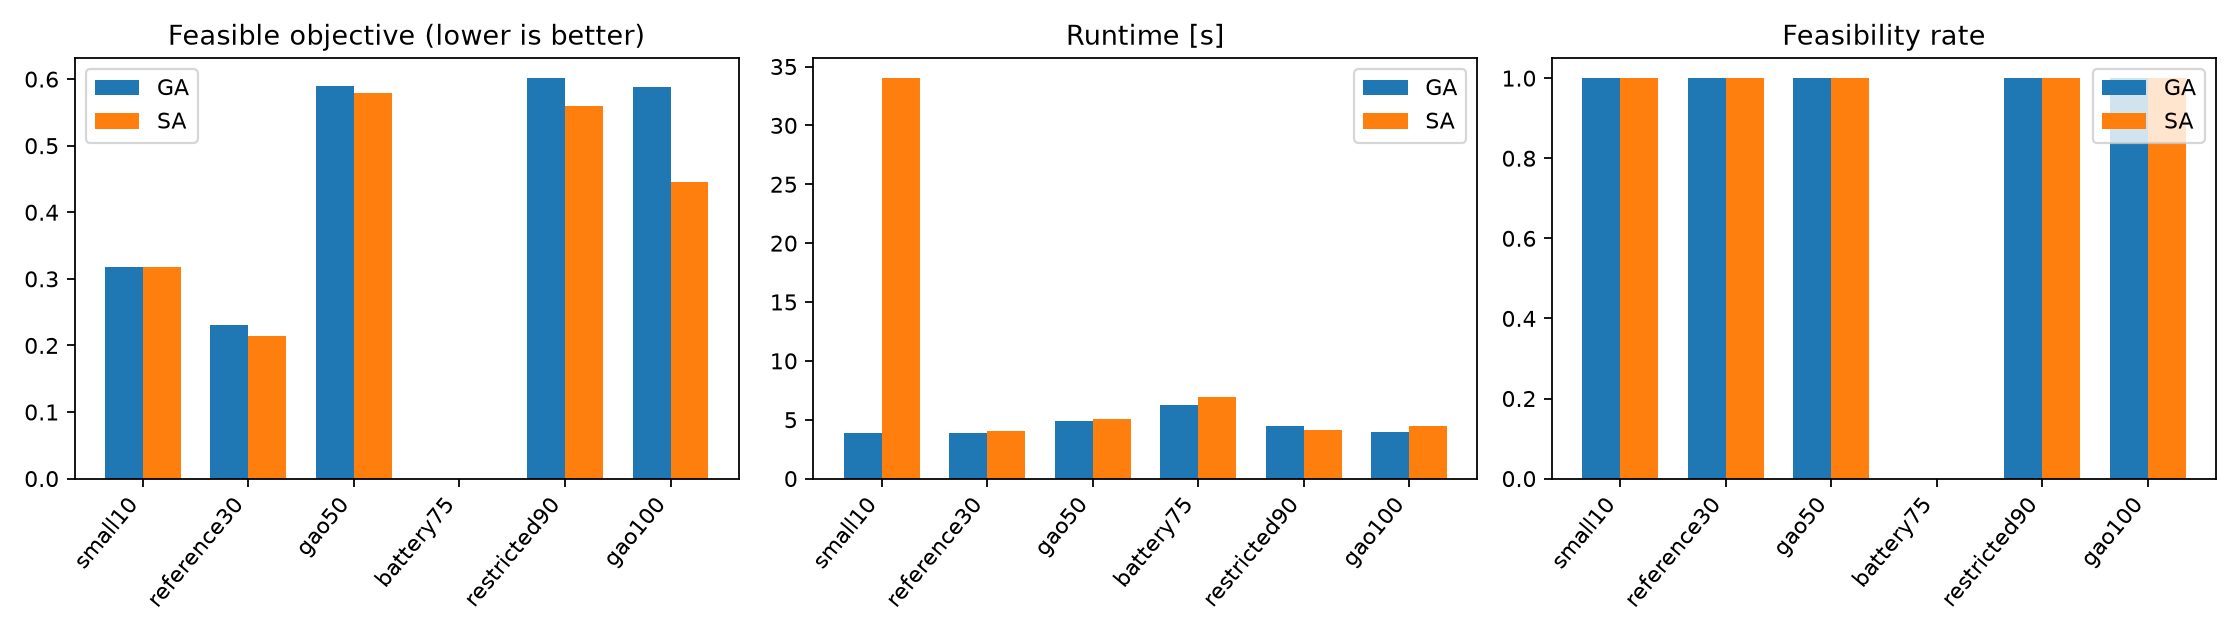
\includegraphics[width=\textwidth]{Figures/milestone4/comparison.png}\caption{GA and SA comparison over five solver seeds.}\end{figure}
\begin{figure}[htbp]\centering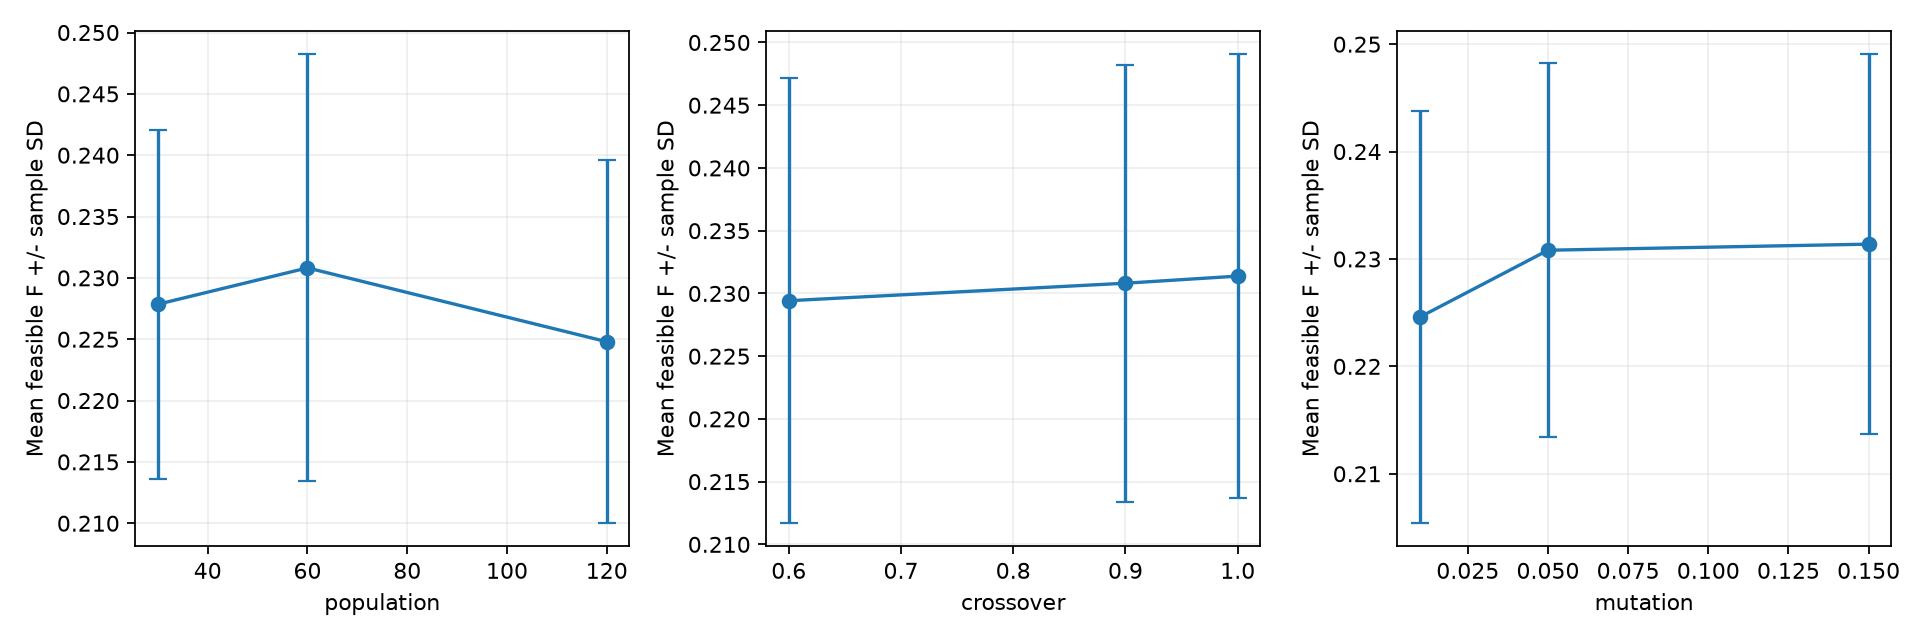
\includegraphics[width=\textwidth]{Figures/milestone4/parameters.png}\caption{One-factor GA studies with sample standard deviations.}\end{figure}
\begin{figure}[htbp]\centering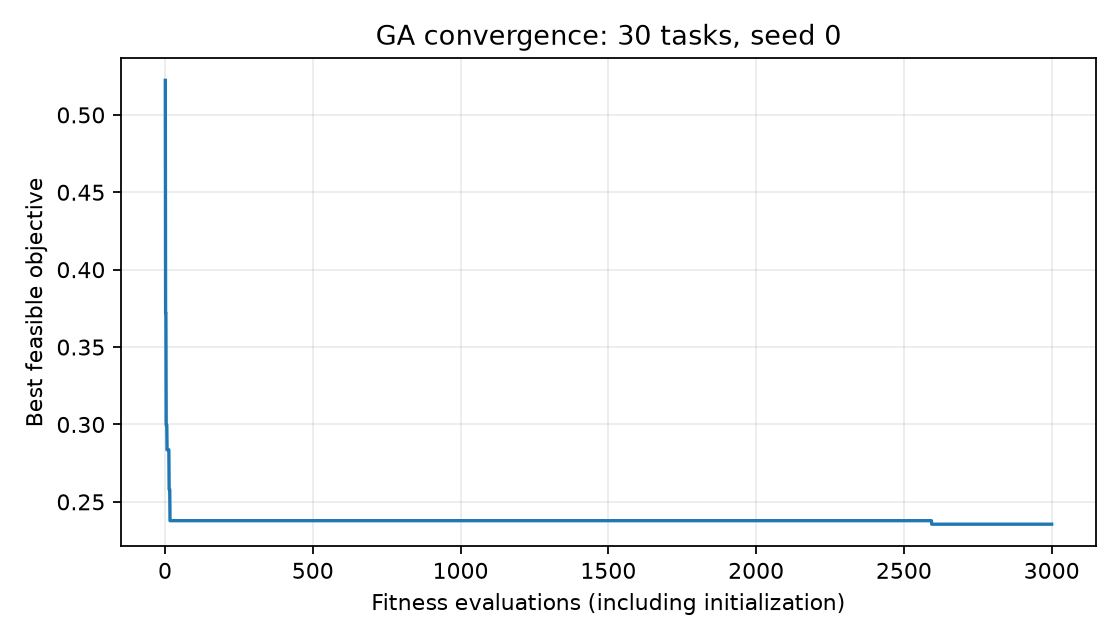
\includegraphics[width=\textwidth]{Figures/milestone4/ga_convergence.png}\caption{Example GA convergence including initialization work.}\end{figure}
\begin{figure}[htbp]\centering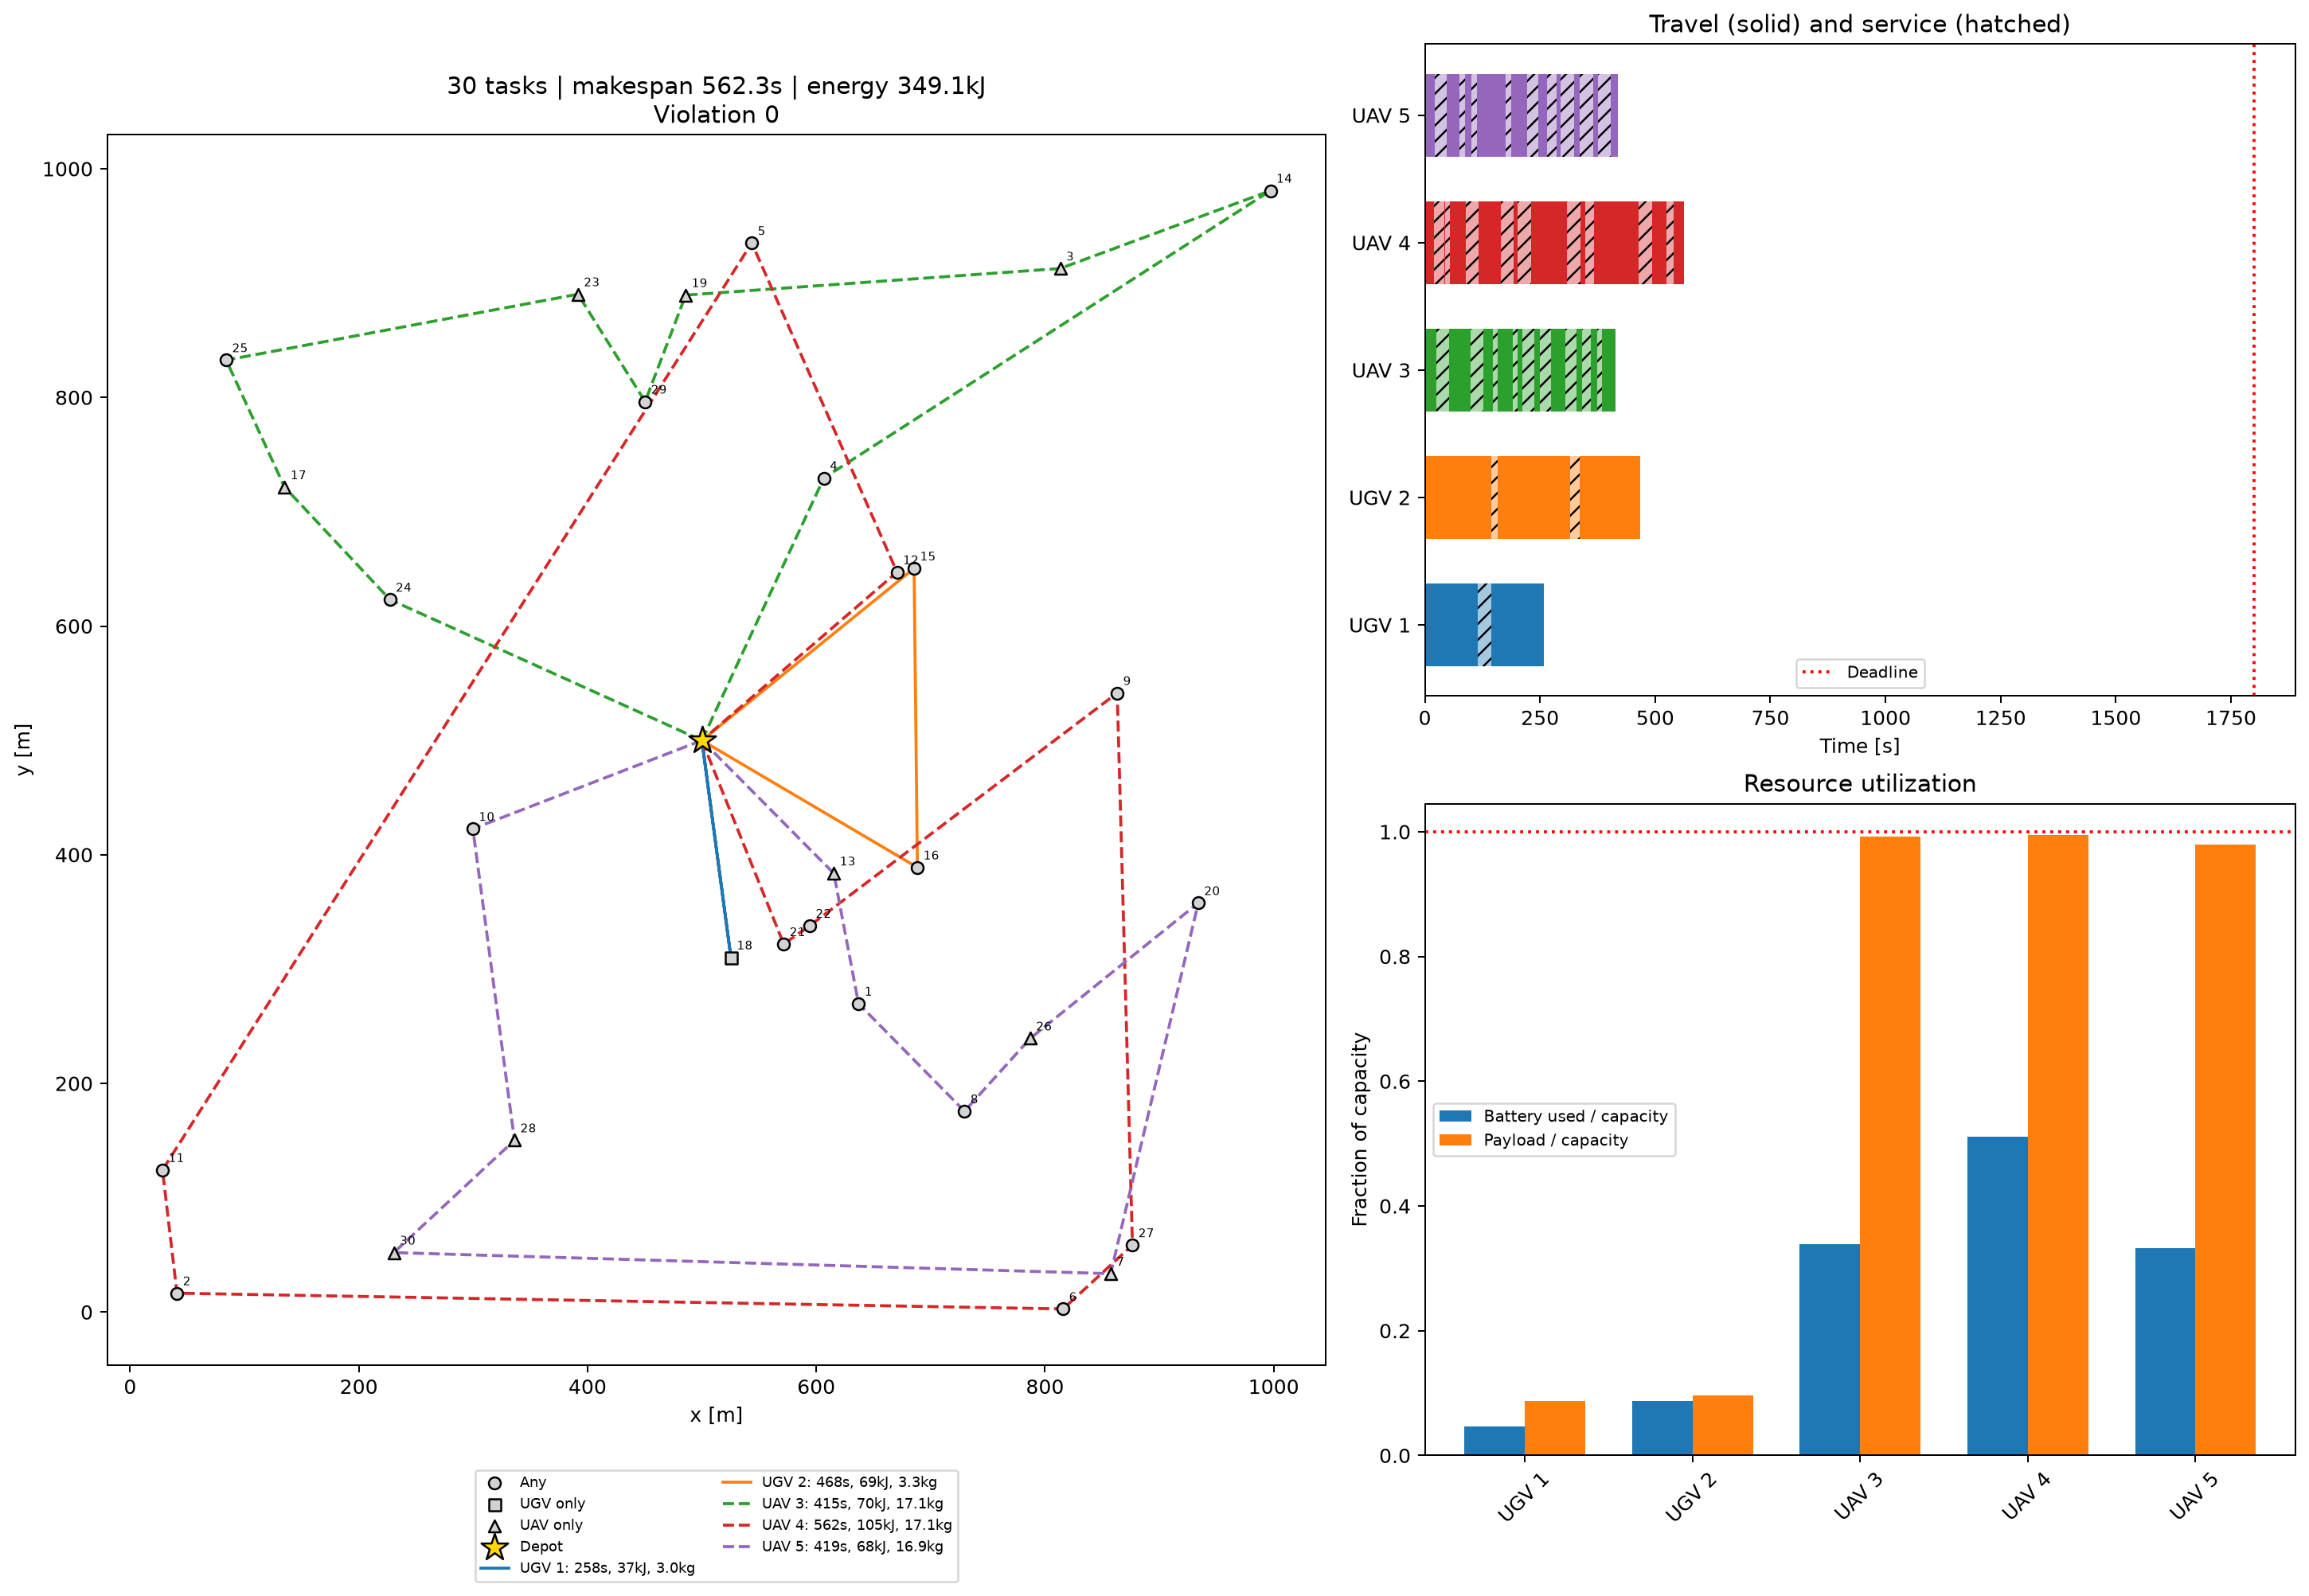
\includegraphics[width=\textwidth]{Figures/milestone4/reference30_GA_routes.png}\caption{GA solution for the 30-task instance, seed zero.}\end{figure}
\section{Discussion and limitations}
Compare feasibility before comparing objective values. A low objective on an infeasible route is not a valid improvement. Mission makespan and energy are the two primary problem-specific performance indices; runtime and feasibility provide additional context. Sample standard deviations and raw repeats are supplied in summary.json and runs.csv.
Increasing population under a fixed evaluation budget reduces the available number of generations. Mutation can restore diversity but can also disrupt useful allocation and order genes. The one-factor study does not establish parameter interactions or a universal best configuration. Repeated solver seeds on one instance measure search variation, not generalization across independent instances.
The exact-instance gap measures distance from a proven optimum. For larger cases no optimality certificate is claimed. Conclusions apply only to these instances, seeds and computational budgets. NumPy and Matplotlib are allowed dependencies, as confirmed by the team. No optimization toolbox implements either solver.